%-------------------------------------------------
% FileName: prac-note.tex
% Author: 
% Version: 1.0
% Description: 实践记录（对齐送花系统规格书格式）
%------------------------------------------------- 

% 断页
\clearpage

% 修复章节编号层级（section无前置0、层级规范）
\renewcommand{\thesection}{\arabic{section}}
\renewcommand{\thesubsection}{\thesection.\arabic{subsection}}
\renewcommand{\thesubsubsection}{\thesubsection.\arabic{subsubsection}}

% 目录深度 & 编号深度
\setcounter{tocdepth}{3}
\setcounter{secnumdepth}{3}

% 生成目录
\tableofcontents
\newpage

\chapter{软件需求规格说明书}

\section{概述}
\subsection{目的}
编写本文档旨在统一项目参与各方对系统业务功能与软件需求的认知，作为项目设计、开发、测试、交付与维护的统一依据。
本文档可作为项目组成员快速熟悉业务的参考资料，同时为后续系统迭代、功能改造、版本升级提供标准化文档支撑。

\subsection{范围}
本文档针对「AI心理健康助手平台」Web 系统及后台管理子系统进行需求定义，包含用户端功能、管理员运维功能、AI 交互能力、数据记录与权限管控等全部业务场景。

\subsection{定义、缩略语及缩写}
本文档无特殊专业定义、缩略语与专用缩写说明。

\subsection{参考资料}
本文档无外部参考资料。

\subsection{文档概貌}
本文档依次阐述系统整体概述、参与者角色、核心用例、业务流程、约束条件与非功能需求，通过用例模型完整描述用户与系统的交互逻辑，结合功能性与非功能要求，形成完整、规范的软件需求规格说明。

\section{总体说明}
\subsection{用例模型概览}
\subsubsection{系统的参与者（Actors）}
\begin{itemize}
    \item 访客：未注册匿名用户，仅可访问平台公开内容与公共资讯。
    \item 注册用户：完成账号注册并正常登录的使用者，可使用 AI 咨询、情绪日记、知识库查阅等核心业务功能。
    \item 管理员：平台运营与运维管理人员，负责内容维护、用户数据查看、风险内容监测与后台管控。
\end{itemize}

\subsubsection{系统主要用例}
\textbf{登录系统}

参与者：注册用户、管理员。
用户进入登录页面填写账号与密码并提交，系统完成身份校验，校验通过后按角色权限跳转对应首页；校验失败则给出标准化错误提示。

\textbf{浏览平台内容}

参与者：访客、注册用户。
所有访问者均可正常浏览平台首页、心理健康科普资讯、公开知识库文章，查看内容详情与基础分类信息。

\textbf{用户注册}

参与者：访客。
匿名访客通过填写基础账号信息完成账号注册，系统校验字段合法性与唯一性，完成账号初始化与基础档案创建。

\textbf{AI咨询聊天}

参与者：注册用户。
登录用户进入智能咨询模块，与 AI 心理健康助手进行实时对话交互，系统统一管理会话上下文并持久化保存咨询记录。

\textbf{记录情绪日记}

参与者：注册用户。
用户自主填写情绪状态、压力水平、生活事件、睡眠情况等个人心理数据，形成长期情绪档案，用于自我监测与后台风险筛查。

\textbf{浏览知识库}

参与者：访客、注册用户。
支持按分类、关键词检索心理科普文章，提供分页浏览、内容阅读等基础资讯服务。

\textbf{管理文章}

参与者：管理员。
后台管理人员对知识库文章执行新增、编辑、上下架、删除等全生命周期内容管理操作。

\textbf{查看咨询记录}

参与者：管理员。
管理员在权限范围内查看全体用户 AI 咨询会话列表、对话内容与访问时间，支持多条件筛选与分页查询。

\textbf{查看情绪记录}

参与者：管理员。
集中查看用户提交的情绪日记数据，结合风险标签识别高危心理状态，为平台风控与人文关怀提供数据支撑。

\subsubsection{用例视图}
本平台用例视图围绕访客、注册用户、管理员三类核心参与者构建，完整呈现不同角色与系统功能的关联关系，明确权限边界与业务交互范围。

\begin{figure}[h]
    \centering
    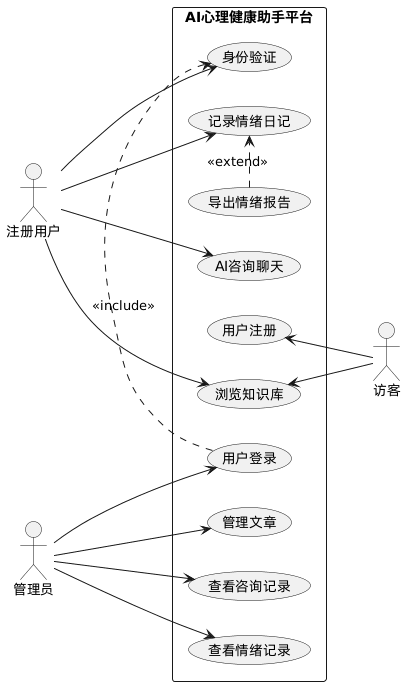
\includegraphics[width=0.8\textwidth]{plantuml.png}
    \caption{AI心理健康助手平台用例图}
\end{figure}

\subsection{假设与依赖}
\begin{enumerate}
    \item 系统权限分级管控，访客仅开放公开浏览权限，注册用户解锁全部核心业务功能。
    \item 用户隐私数据、聊天记录、情绪档案均采用加密存储，保障个人信息安全合规。
    \item 智能对话功能依赖第三方 AI 接口服务，接口可用性直接影响咨询模块运行状态。
    \item 本次迭代暂不接入第三方登录、在线支付、消息推送等扩展业务。
\end{enumerate}

\section{具体需求}
\subsection{用例报告}

\subsubsection{公共用例}

\par
\indent 用例名：用户登录
\par
\indent 参与者：注册用户、管理员
\par
\indent 前置条件：系统已完成部署，数据库存在合法账号数据
\par
\indent 后置条件：校验通过后记录用户登录会话，授予对应角色操作权限
\par
\indent 主要流程：
\begin{enumerate}
    \item 用户进入系统登录界面；
    \item 填写账号、密码并提交登录请求；
    \item 系统校验账号密码合法性；
    \item 校验通过，按用户角色跳转至对应功能主页。
\end{enumerate}
\par
\indent 变化流程：
\begin{itemize}
    \item 2a 表单信息填写不完整：系统高亮提示必填项，停留登录页面；
    \item 3a 账号或密码不匹配：统一返回权限错误提示，防止暴力破解；
    \item 3b 账户被禁用：系统提示账户已被禁用，请联系管理员，用例终止。
\end{itemize}

\par
\indent 用例名：浏览知识库
\par
\indent 参与者：访客、注册用户
\par
\indent 前置条件：用户成功访问平台知识库模块
\par
\indent 后置条件：用户获取心理健康知识
\par
\indent 主要流程：
\begin{enumerate}
    \item 系统展示文章分类目录与图文列表；
    \item 支持分类筛选、关键词检索快速定位内容；
    \item 点击文章条目查看完整科普内容；
    \item 累计统计内容阅读量。
\end{enumerate}
\par
\indent 变化流程：
\begin{itemize}
    \item 2a 按分类筛选：显示对应分类文章；
    \item 2b 关键词搜索：显示匹配结果；
    \item 4a 切换分页：加载对应页内容。
\end{itemize}

\subsubsection{访客用例}

\par
\indent 用例名：用户注册
\par
\indent 参与者：访客
\par
\indent 前置条件：访客成功访问系统注册页面
\par
\indent 后置条件：系统生成独立用户账号，写入基础用户数据表
\par
\indent 主要流程：
\begin{enumerate}
    \item 访客进入注册界面；
    \item 按规范填写用户名、邮箱、密码、确认密码等必填字段；
    \item 系统校验字段格式、长度规则与数据唯一性；
    \item 校验无误后加密保存用户信息，提示注册成功并跳转登录页。
\end{enumerate}
\par
\indent 变化流程：
\begin{itemize}
    \item 2a 字段格式非法、长度超限：实时格式校验并给出修改指引；
    \item 2b 用户名或邮箱已被占用：提示冲突信息，引导更换内容；
    \item 4a 信息填写不完整：系统提示“请填写所有必填项”，返回步骤2。
\end{itemize}

\subsubsection{注册用户用例}

\par
\indent 用例名：AI咨询聊天
\par
\indent 参与者：注册用户
\par
\indent 前置条件：用户已完成登录，会话状态正常
\par
\indent 后置条件：单次对话内容自动归档至个人咨询记录
\par
\indent 主要流程：
\begin{enumerate}
    \item 登录用户进入 AI 智能咨询模块；
    \item 加载历史会话记录与聊天交互界面；
    \item 用户编辑并提交咨询内容；
    \item 系统调用 AI 服务接口获取应答数据；
    \item 渲染 AI 回复内容，同步保存完整会话。
\end{enumerate}
\par
\indent 变化流程：
\begin{itemize}
    \item 3a 使用快捷提示：系统自动填入并发送，继续步骤4；
    \item 4a 上游 AI 接口响应超时：提示服务繁忙，支持重试操作；
    \item 4b 识别到极端负面、自残、抑郁等高风险内容：自动标记预警并展示心理援助渠道。
\end{itemize}

\par
\indent 用例名：记录情绪日记
\par
\indent 参与者：注册用户
\par
\indent 前置条件：用户已正常登录系统
\par
\indent 后置条件：情绪表单数据持久化存储，纳入个人健康档案
\par
\indent 主要流程：
\begin{enumerate}
    \item 用户进入情绪日记填写页面；
    \item 选择当日情绪评分、情绪标签；
    \item 补充生活事件、内心想法、睡眠质量、压力等级等描述信息；
    \item 提交表单，系统完成数据校验与入库；
    \item 页面反馈保存成功提示。
\end{enumerate}
\par
\indent 变化流程：
\begin{itemize}
    \item 2a 未选择核心必填项：拦截提交操作，标注缺失字段；
    \item 3a 用户清空表单：重置所有内容，返回步骤2。
\end{itemize}

\subsubsection{管理员用例}

\par
\indent 用例名：管理文章
\par
\indent 参与者：管理员
\par
\indent 前置条件：管理员完成后台登录，拥有内容管理权限
\par
\indent 后置条件：文章内容完成新增、修改或下架删除，数据实时生效
\par
\indent 主要流程：
\begin{enumerate}
    \item 管理员进入后台内容管理模块；
    \item 系统展示全部知识库文章列表；
    \item 执行新增发布、编辑内容、修改状态或删除操作；
    \item 后台校验数据合规性，更新数据库并刷新列表。
\end{enumerate}
\par
\indent 变化流程：
\begin{itemize}
    \item 3a 关键内容缺失或格式违规：禁止提交并给出修改提示；
    \item 3b 删除文章：二次确认后删除并刷新列表。
\end{itemize}

\par
\indent 用例名：查看咨询记录
\par
\indent 参与者：管理员
\par
\indent 前置条件：管理员已登录后台系统
\par
\indent 后置条件：可完整查阅指定用户历史咨询会话
\par
\indent 主要流程：
\begin{enumerate}
    \item 管理员进入咨询记录管理页面；
    \item 系统按时间倒序展示全部会话摘要；
    \item 支持按用户ID、时间区间多条件筛选；
    \item 点开详情查看完整对话上下文。
\end{enumerate}
\par
\indent 变化流程：
\begin{itemize}
    \item 3a 关键词检索指定用户，精准定位目标记录；
    \item 3b 分页浏览：切换页码加载数据。
\end{itemize}

\par
\indent 用例名：查看情绪记录
\par
\indent 参与者：管理员
\par
\indent 前置条件：管理员已登录后台系统
\par
\indent 后置条件：获取用户长期情绪变化数据与风险标签
\par
\indent 主要流程：
\begin{enumerate}
    \item 管理员进入情绪数据统计页面；
    \item 系统批量展示用户情绪日记列表；
    \item 按风险等级、提交时间、用户维度筛选数据；
    \item 高危情绪记录特殊高亮标记，便于重点关注。
\end{enumerate}
\par
\indent 变化流程：
\begin{itemize}
    \item 3a 按风险等级筛选：显示低/中/高风险记录；
    \item 3b 按日期范围筛选：显示指定时间段记录；
    \item 4a 高风险记录：红色警示突出显示。
\end{itemize}

\section{补充需求}
\subsection{功能性需求补充}
\begin{itemize}
    \item 知识库文章分类统一后台配置，支持动态新增、编辑分类，无需修改代码重启服务。
    \item 严格数据权限隔离，普通用户仅可见个人数据，管理员仅在授权范围内查看公共运营数据，杜绝越权访问。
    \item 系统内置敏感词与风险内容识别机制，对暴力、消极、自残、极端言论自动拦截、标记与预警。
    \item 会话记录、情绪日记支持长期归档存储，保留历史数据，便于后期统计分析与系统优化。
    \item 前端路由权限拦截，未登录用户访问受限页面自动强制跳转登录界面。
\end{itemize}

\subsection{可用性需求}
界面布局简洁统一，操作逻辑清晰，功能命名通俗易懂；
关键操作配有文字提示、表单校验与错误指引，降低使用门槛；
整体交互风格统一，适配主流浏览器访问，保证不同终端基础使用体验一致。

\subsection{可靠性需求}
系统服务持续稳定运行，全年可用率不低于 99\%；
核心业务数据采用持久化存储，关键操作加入事务控制，避免数据丢失、重复写入或异常错乱；
异常场景具备容错处理，接口异常、网络波动时友好提示，避免页面崩溃。

\subsection{性能需求}
普通页面常规加载响应时间控制在 2 秒以内；
AI 咨询接口应答响应时间不超过 3 秒；
系统支持至少 100 名用户同时在线正常访问，高峰期服务无明显卡顿；
列表数据采用分页懒加载机制，减少一次性数据渲染压力。

\subsection{安全性需求}
用户登录密码加密存储，传输过程采用安全协议加固；
前后端双重表单校验，防范非法参数、恶意提交与注入攻击；
后台管理员操作留痕，关键管理行为记录操作日志，便于溯源审计；
用户隐私数据脱敏展示，禁止明文泄露敏感个人信息。

\subsection{可维护性需求}
前后端业务模块解耦，代码结构分层清晰，便于后期迭代开发；
系统关键配置集中管理，参数可动态调整，降低运维成本；
统一异常捕获与日志输出，问题可快速定位、排查与修复；
文档与代码同步更新，保障项目交接与长期维护。

\subsection{兼容性需求}
适配 Chrome、Edge、360 等主流现代浏览器；
页面采用自适应布局，兼容电脑端常规分辨率展示；
接口格式标准化，便于后续对接小程序、移动端 H5 等多端扩展。

\subsection{设计与约束需求}
\begin{itemize}
    \item 整体视觉风格贴合心理健康产品定位，色调温和简约，弱化强刺激元素。
    \item 业务流程遵循最简操作原则，减少冗余步骤，提升用户使用体验。
    \item 严格遵循本次项目开发范围，不额外扩展非约定业务功能。
    \item 所有功能设计符合网络内容规范与青少年心理健康引导要求。
\end{itemize}